\documentclass[svgnames,11pt]{beamer}
\input{/home/tof/Documents/Cozy/latex-include/preambule_commun.tex}
\input{/home/tof/Documents/Cozy/latex-include/preambule_beamer.tex}
%\usepackage{pgfpages} \setbeameroption{show notes on second screen=left}
\author[]{Christophe Viroulaud}
\title{Géocube mesures}
\date{\framebox{\textbf{Donn 02}}}
%\logo{}
\institute{Seconde - SNT}

\begin{document}
\begin{frame}
\titlepage
\end{frame}
\begin{frame}
    \frametitle{}
    \begin{center}
    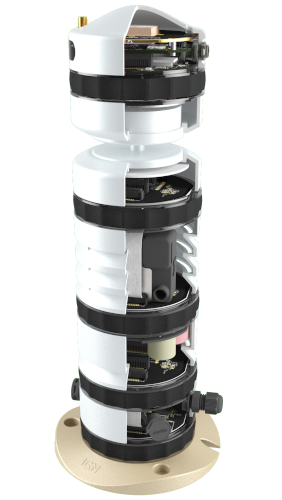
\includegraphics[width=3cm]{ressources/geocube-interne.png}
    \captionof{figure}{Le Géocube effectue de nombreuses mesures par jour.
    }
    \end{center}

\end{frame}
\begin{frame}
    \frametitle{}

    \begin{framed}\centering
        Comment manipuler de grandes quantités de données? 
    \end{framed}

\end{frame}
\section{Stocker des données}
\begin{frame}
    \frametitle{Stocker des données}
    Les données fournies par le Géocube sont stockées dans un fichier \emph{csv}.
    \begin{center}
        nom,prenom,naissance\\
        Dupont,John,2006-12-09\\
        Durant,James,2008-06-10
    \end{center}
\begin{aretenir}[]
    Un fichier \textbf{csv (Comma Separated Values)} stocke les données sous forme de tableau. Une donnée est caractérisée par ses \textbf{descripteurs}. \\
    Chaque valeur est séparée par un caractère spécial: une virgule, un point-virgule, une tabulation\dots
\end{aretenir}   

\end{frame}
\begin{frame}
    \frametitle{}

    \begin{activite}
    \begin{enumerate}
        \item Sur le site \url{https://geobs.fr/cartograph/} trouver le Géocube GV6\_0025 placé à l'IGN (sud-est de Paris).
        \item Cliquer sur \textbf{\texttt{Ajouter}} puis \textbf{\texttt{Voir les données}}.
        \item Sélectionner la température et la pression sur l'intervalle du 1 septembre 2021 à aujourd'hui. Appliquer les modifications.
        \item Télécharger les fichiers \textbf{\texttt{csv}} pour chaque donnée.
    \end{enumerate}
    \end{activite}

\end{frame}
\begin{frame}
    \frametitle{Avant de regarder la correction}
\begin{center}
    \centering
    \includegraphics[width=3cm]{/home/tof/Documents/Cozy/latex-include/stop.png}
    \end{center}
{\Large
    \begin{itemize}
        \item Prendre le temps de réfléchir,
        \item Analyser les messages d'erreur,
        \item Demander au professeur.
    \end{itemize}
}
\end{frame}
\begin{frame}
    \frametitle{Correction}

    \begin{center}
        En cas de problème télécharger le dossier compressé 
        \href{https://cviroulaud.github.io/seconde/donnees/geocube-mesures/ressources/donnees-0025.zip}{en cliquant ici}.
    \end{center}

\end{frame}
\begin{frame}
    \frametitle{}

    

\end{frame}
\section{Manipuler des données}
\end{document}